\documentclass[journal]{IEEEtran}

%\usepackage[retainorgcmds]{IEEEtrantools}
%\usepackage{bibentry}  
\usepackage{xcolor,soul,framed} %caption

\colorlet{shadecolor}{yellow}
% \usepackage{color,soul}
\usepackage[pdftex]{graphicx}
\graphicspath{{../photo/}}
\DeclareGraphicsExtensions{.pdf,.jpeg,.png}
\usepackage[caption=false]{subfig}
\usepackage[cmex10]{amsmath}
\usepackage{amssymb}
\usepackage{array}
\usepackage{mdwmath}
\usepackage{mdwtab}
\usepackage{eqparbox}
\usepackage{cite}
\usepackage{tabularx,booktabs}
\usepackage[flushleft]{threeparttable} % table notes
\usepackage{algorithm,algorithmic}
\usepackage{footmisc}
\usepackage[colorlinks=true]{hyperref}
\hypersetup{
    citecolor = black,
    urlcolor = blue
}

\hyphenation{op-tical net-works semi-conduc-tor}

%\bstctlcite{IEEE:BSTcontrol}

% === TITLE & AUTHORS ===================================================
% =======================================================================
\begin{document}
\bstctlcite{IEEEexample:BSTcontrol}
    \title{Simulation Modeling of Glycosylation Effects on Potassium Channels of Mouse Cardiomyocytes}
  \author{Haedong Kim,~\IEEEmembership{{Student Member},~IEEE,}
      Hui Yang,~\IEEEmembership{Senior Member,~IEEE,}
      Andrew R. Ednie,
      and~Eric S. Bennett
  \thanks{Manuscript received Month Day, Year}
  \thanks{H. Kim and H. Yang are with the Complex Systems Monitoring, Modeling, and Control Laboratory, The Pennsylvania State University, University Park, PA 16802 USA (e-mail: huk344@psu.edu; huy25@psu.edu).}% <-this % stops a space
  \thanks{A. R. Ednie and E. S. Bennett are with the Department of Neuroscience, Cell Biology and Physiology, Wright State University, Dayton, OH 45435 USA (e-mail: andrew.ednie@wright.edu; eric.bennett@wright.edu).}}

% The paper headers
% The only time the second header will appear is for the odd numbered pages after the title page when using the two-side option.
\markboth{}%
{Kim \MakeLowercase{\textit{et al.}}: Potassium Channel}

% =======================================================================
\maketitle

% === ABSTRACT ==========================================================
% =======================================================================
\begin{abstract}
Cardiovascular disease is a leading cause of death worldwide. Dilated cardiomyopathy (DCM) is the third most common cause of heart failure and the most frequent reason for heart transplantation; upward of 70\% of DCM cases are considered idiopathic. We showed, through in-vitro experiments, that reduced hybrid/complex N-glycosylation in mouse cardiomyocytes is sufficient to cause DCM. Further, we investigated the role of reduced complex N-glycosylation in the gating and activities of voltage-gated ion channels, specifically, the voltage-gated $\text{Na}^{+}$ ($\text{Na}_{v}$), $\text{Ca}^{2+}$ ($\text{Ca}_{v}$), and $\text{K}^{+}$ ($\text{K}_{v}$) channels responsible for ventricular myocyte action potentials (APs). In addition to direct effects of reduced N-glycosylation on $\text{Na}_{v}$ and $\text{Ca}_{v}$ gating, we observed aberrant electrical signalings such as prolonged APs and abnormal early re-activations, consistent with an observed reduction in $\text{K}_{v}$ expression and activity. However, it is difficult to rigorously determine the effects of reduced hybrid/complex N-glycosylation on $\text{K}_{v}$ activity, as there are multiple isoforms in the mouse ventricle including, $\text{K}_{v}1.5$, $\text{K}_{v}2.1$, and $\text{K}_{v}4.2$, that collectively produce the repolarizing phase of the AP. Experimentally, because of the unique inactivation kinetics of the $\text{K}_{v}$ isoforms, only the sum of $\text{K}^{+}$ currents ($\text{I}_{Ksum}$) can be recorded and decomposed into component currents using exponential fitting to estimate the currents flowing through $\text{K}_{v}$ isoforms. However, such decomposition cannot describe effectively the mechanism of $\text{K}_{v}$ under different conditions. Here, we propose the use of simulation models to describe statistics and data recorded from in-vitro experiments. We developed simulation models for dominant $\text{K}^{+}$ currents in mouse ventricular myocytes and calibrate their parameters using the in-vitro data under normal and reduced glycosylation conditions through ablation of the Mgat1 gene. A novel model calibration procedure is proposed to deal with the complex structure of the ionic current models based on nonlinear functions and differential equations. Experimental results show that the proposed method has strong potential to build complex simulation models with sparse data and predict characteristics of multiple $\text{K}_{v}$ isoforms to understand detailed kinetics.
\end{abstract}

% === KEYWORDS ==========================================================
% =======================================================================
\begin{IEEEkeywords}
Electrophysiology, N-glycosylation, dilated cardiomyopathy, voltage-gated potassium channel, simulation modeling, genetic algorithm. 
\end{IEEEkeywords}

% For peer review papers, you can put extra information on the cover
% page as needed:
% \ifCLASSOPTIONpeerreview
% \begin{center} \bfseries EDICS Category: 3-BBND \end{center}
% \fi
%
% For peerreview papers, this IEEEtran command inserts a page break and
% creates the second title. It will be ignored for other modes.
\IEEEpeerreviewmaketitle

% === I. INTRODUCTION ===================================================
% =======================================================================
\section{Introduction}
\IEEEPARstart{H}{eart} disease is the leading cause of death globally, accounting for 23\% of deaths in the U.S. in 2017 \cite{cdc2019deaths}. Dilated cardiomyopathy (DCM) is one of the most common cause of heart failure that calls for heart transplantation \cite{weintraub2017dilated}. DCM is characterized by enlarged and weakened ventricular chambers, and it is associated with systolic and contractile dysfunction that has a high risk to heart failure, with approximately 70\% of DCM cases regarded as idiopathic \cite{weintraub2017dilated, lakdawala2013dilated, hershberger2011update}. There has been consistent and increasing evidence of a link between aberrant glycosylation and heart failure \cite{barrans2002global, hwang2002microarray, yung2004gene, nishio1995identification, knezevic2009variability, miura2016glycomics, nagai2016aberrant, yang2015glycoproteins, jacob2013altered, ufret2001role, gehrmann2003cardiomyopathy, marques2017cardiac}. Recently, we showed that reduction of hybrid/complex N-glycosylation in mouse cardiomyocytes through ablation of the Mgat1\footnote{Mannosyl ($\alpha$-1,3-)-Glycoprotein $\beta$-1,2-N-acetylglucosaminyltransferase} gene that encodes a critical glycosyltransferase (GlcNAcT1\footnote{UDP-GlcNAc:$\alpha$-3-D-mannoside-$\beta$1,2-N-acetylglucosaminyltransferase}) (Mgat1KO model), is sufficient to cause DCM \cite{ednie2019reduced, ednie2019reduced2}. Mgat1KO mice develop DCM, heart failure, and 100\% die early, likely from ventricular arrhythmias resulting in sudden cardiac death. Further, Mgat1KO ventricular myocytes demonstrated altered electromechanical functions, including excitation-contraction (EC) coupling and contraction consistencies with observed changes in electrical signaling caused by acute and downstream (disease-related) effects on voltage-gated ion channel (VGIC) gating and activity \cite{ednie2019reduced}. 

Thus, we investigated the impact of reduced hybrid/complex N-glycosylation through the lens of electrophysiology. Electrophysiology refers to studies of electrical properties in cells, tissues, or organs, including the examination of voltage, currents, and changes in scales from ion channels to organ systems \cite{scanziani2009electrophysiology}. Electrical signaling in the heart has vital functions related to intra and extracellular communication, rhythmicity of heartbeats, and provides a driving force for contraction. The action potential (AP) is the net transmembrane potential varying over time which results from the composite activities of different ion channels \cite{grant2009cardiac}. Fig. 1-(a) shows the simulated AP of a mouse ventricular apex myocyte using models adopted from \cite{bondarenko2004computer}. The AP is the result of orchestrated activities of various ionic currents described in Fig. 1-(b). Even small changes in VGIC's function can contribute to aberrant AP waveform and/or conduction, leading to arrhythmias. As illustrated in Fig. 2, voltage-gated $\text{Na}^{+}$ channels ($\text{Na}_{v}$) are responsible for AP initiation, or the depolarization phase, voltage-gated $\text{Ca}^{2+}$ channels ($\text{Ca}_{v}$) are responsible for the prolonged depolarization phase particularly in larger species (“plateau”), while several voltage-gated $\text{K}^{+}$ channel ($\text{K}_{v}$) isoforms are collectively responsible for AP deactivation, i.e., repolarization. Like most transmembrane proteins, VGICs are heavily glycosylated membrane proteins \cite{ednie2011modulation}. Studies have proven that glycosylation can affect VGIC function predominantly. For example, we reported that a saturating, electrostatic effect of negatively charged sialic acids, which are typically attached to the terminal of glycan branches, significantly altered cardiac electrical signaling \cite{ednie2013expression, ednie2015reduced}. In our recent studies \cite{ednie2019reduced, ednie2019reduced2}, we observed, for Mgat1KO ventricular apex myocytes, aberrant electrical signaling such as prolonged APs and abnormal early re-activations, caused by direct and disease-related effects of reduced N-glycosylation on VGIC gating and activity that are consistent with the AP waveform and conduction anomalies observed.
\begin{figure}
    \label{fig1}
    \centering
    \subfloat[]{\includegraphics[width=0.8\linewidth]{photo/sim_ap.png}}
    \\
    \subfloat[]{\includegraphics[width=0.8\linewidth]{photo/sim_currents.png}}
    \caption{Simulation results of the (a) action potential and (b) relevant ionic currents (i.e., $\text{I}_{Kto}$, $\text{I}_{Kslow}$, $\text{I}_{Kss}$, $\text{I}_{Na}$, and $\text{I}_{CaL}$) of mouse ventricular myocytes. Potassium currents have positive currents, while sodium and calcium currents are negative.}
\end{figure}

\begin{figure}
    \label{fig2}
    \centering
    \includegraphics[width=0.8\linewidth]{photo/ap_ion_channels.png}
    \caption{Predominant ion channels in human ventricular myocytes and their functional role in shaping an AP}
    \label{fig:my_label}
\end{figure}

Although these in-vitro experiments showed changes in activities of ion channels, there are certain limitations that include: 1) \textit{Detailed ion channel kinetics are difficult to determine rigorously using in-vitro experiments alone}. From the electrophysiological experiment, pathological electrical signaling can be observed through measurements of APs at the whole-cell level and currents at the ion-channel level. However, it is difficult to relate, rigorously, the impacts of VGIC gating changes to the altered AP waveform/conduction and vice versa. 2) \textit{Segregating different $\text{K}^{+}$ currents ($\text{I}_{K}$) is difficult using whole-cell recording experimental techniques only}. $\text{I}_{Ksum}$ is the result of activity of multiple isoforms with each isoform producing a different, but slightly overlapping (in activation and inactivation voltages) component of the total $\text{K}^{+}$ current ($\text{I}_{Ksum}$) \cite{brouillette2004functional} that thereby contributes to various portions of AP repolarization. However, in-vitro experiments can only measure the sum of these component currents ($\text{I}_{Ksum}$) using whole-cell voltage-clamp protocols. Even pharmacologic separation of $\text{K}_{v}$ current types is difficult, as the specificity of drugs for a single current type is not ideal. Therefore, component $\text{K}^{+}$ currents are usually estimated through multiple exponential fits of the decaying portion (due to channel inactivation) of the total $\text{K}^{+}$ current \cite{brunet2004heterogeneous}. Although the exponential function illustrates the shape of a component-current trace well, it cannot adequately describe kinetic dynamics of the current, nor fully and rigorously distinguish among currents produced by different $\text{K}_{v}$ isoforms because of their slightly overlapping voltage-dependence of gating. As $\text{K}_{v}$ have a critical function in repolarizing the cell, it is imperative to examine $\text{K}_{v}$ isoform thoroughly.

Therefore, in this study, we propose mathematical simulation methods to model different $\text{K}^{+}$ component currents so that $\text{I}_{Ksum}$ is decomposed to study two major voltage-dependent component $\text{K}^{+}$ currents with simulation models, $\text{I}_{Kto}$ and $\text{I}_{Kslow}$. Fig. 3 shows an example of the major component $\text{K}^{+}$ currents with the sum $\text{K}^{+}$ current shown as a red-solid line. Except for the $\text{K}^{+}$ steady-state current ($\text{I}_{Kss}$) component, $\text{K}^{+}$ currents have the shape of reaching the peak relatively early following a depolarization that decreases at variable rates. Thus, there are two critical measures for the shape of $\text{K}^{+}$ current traces: peak value and the current attenuation. As reported in \cite{ednie2019reduced}, we derived key statistics of the component currents, amplitudes, and inactivation rates ($\tau$'s) using bi-exponential fits from the $\text{I}_{Ksum}$ traces of the in-vitro experimental data measured following a 4.5 s stimulus depolarizing pulse. Amplitude and $\tau$ refer to the value of the peak and the time constant when current reduces by $e^{-1}$ (almost 63\%) of the peak. These key statistics were used to calibrate biophysical simulation models. The outcomes and impacts of this research are summarized as follows.
\begin{itemize}
    \item Detailed $\text{K}_{v}$ kinetics can be simulated and predicted using the proposed model to get a better understanding of $\text{K}_{v}$ kinetics, unlike an exponential function, which only describes a current trace.
    \item The simulation models can be fitted to current trace data directly, from which the differences across observations, i.e., cells, can be characterized.
\end{itemize}

% === II. RESEARCH BACKGROUND ===========================================
% =======================================================================
\section{Research Background}
\subsection{Glycosylation and DCM}
Protein glycosylation is an essential cellular process that impacts many cell functions \cite{marques2017cardiac}. Briefly, protein glycosylation is the sequential co-/post-translational process of attaching sugar residues (glycans) to proteins. Cardiac VGICs are heavily glycosylated proteins with upwards of 30\% of their mass consisting of N- and O-linked glycans. A growing number of cardiac diseases, including DCM and hypertrophic cardiomyopathy, can present with concurrent, albeit, modest changes in glycosylation \cite{gehrmann2003cardiomyopathy, footitt2009cardiomyopathy, marques2017cardiac}. Mgat1 expression was implicated in cardiac function and shown to be down-regulated in human end-stage idiopathic DCM. Genome-wide searches identified changes in glycosylation-related gene expression in human idiopathic DCM, including glycosyltransferases \cite{barrans2002global, hwang2002microarray, yung2004gene}; and proteomic/glycomic studies show changes in serum N-glycosylation in heart disease models and in humans with DCM risk factors \cite{nishio1995identification, knezevic2009variability, miura2016glycomics, nagai2016aberrant, yang2015glycoproteins}. Models of DCM/heart failure were associated with subtle changes in glycosylation of proteins involved in electromechanical processes, and ~20\% of patients with congenital disorders of glycosylation (CDG) present with cardiac deficits, including idiopathic DCM \cite{gehrmann2003cardiomyopathy, marques2017cardiac}. The data suggest a correlation between modest changes in extracellularly facing glycosylation and DCM/heart disease \cite{yung2004gene, hwang2002microarray, barrans2002global, nagai2016aberrant, yang2015glycoproteins}. 

\subsection{Simulation Modeling of Mouse Ventricular Myocytes}
Electrophysiology was pioneered by Hodgkin and Huxley with a series of famous experiments on the squid giant axon \cite{hodgkin1952quantitative}. Their simulation model was built upon two fundamental principles observed in the experimental data. 1) Cells are selectively activated by different ion channels. 2) Activities of ion channels to produce ionic currents are controlled through voltage changes, from which the name ``voltage-gated ion channels'' originates. The voltage-gating mechanism is embedded in the simulations model by partial differential equations. Not only are simulation models compatible with data and descriptive, but they also simulate changes of action potential waveforms, and cell conductance. Thus, models provide connections among ionic currents, action potentials, and conductance. However, significant domain knowledge in kinetics of ion channels and trial-and-error investigations are required, as advanced cardiomyocyte simulation models have complex structures based on nonlinear functions and differential equations with high dimensionality.

In the literature, optimization procedures have been proposed to fit cardiomyocyte simulation models to electrophysiological experimental data in an autonomous way as much as possible. $\text{Na}_{v}$ activity was coupled with in-vitro data of mouse cardiomyocyte using fractional factorial design and a Gaussian process model \cite{du2015statistical}. Fractional factorial designs were used to find significant control variables from the entire set of tuning parameters to reduce dimensionality. The Gaussian process model, which is computationally cheaper than the original $\text{Na}_{v}$ model, has served as a surrogate model to find optimal parameters. In \cite{du2017}, $\text{K}^{+}$ component currents, $\text{I}_{Kto}$ ($\text{K}_{v4.2}$ activity), and $\text{I}_{Kslow}$ ($\text{K}_{v1.5}/\text{K}_{v2.1}$ activity) simulation models are calibrated with a nonlinear optimization algorithms, i.e., the trust-region method. 

In both studies, statistics such as steady-state activation (SSA), steady-state inactivation (SSI), and time constant of inactivation at different voltage were used to calculate goodness-of-fit as an objective function of optimization to minimize discrepancies with in-vitro experiment data. However, these characteristic statistics, which are derived from current traces recorded during in-vitro experiments, are not always available. For example, in our Mgat1KO data, currents were too small at early-activating voltages to reliably calculate the characteristic statistics.  

\subsection{$\text{K}_{v}$ Isoforms}
\begin{figure}
    \label{fig3}
    \centering
    \includegraphics[width=0.8\linewidth]{photo/k_decomp_eg.png}
    \caption{Example of $\text{K}^{+}$ current decomposition into three component currents. Each component $\text{K}^{+}$ current has different characteristics in terms of their peak and decaying phase}
\end{figure}
Activation of several different $\text{K}_{v}$ isoforms produces multiple component currents, as illustrated in Fig. 1-(b). However, it is difficult to rigorously delineate the multiple component $\text{K}^{+}$ currents through voltage-clamp experiments alone as the sum of $\text{K}^{+}$ currents is measured \cite{brouillette2004functional}. Thus, $\text{I}_{Ksum}$ is usually decomposed mathematically by fitting the peak and decaying portion of each component current trace with an exponential function \cite{brunet2004heterogeneous}. As given in Equation (1), a standard exponential function has three parameters: amplitude ($\text{A}$), time constant ($\tau$), and constant offset value $\text{C}$. $t$ is time in millisecond. Amplitude refers to the value of the peak and $\tau$ to the time constant when current reduces by $e^{-1}$ (~63\%) of the peak. 

In mouse ventricular myocytes, $\text{I}_{Ksum}$ has often been decomposed into three dominant currents, with one current having a high peak and decaying rapidly ($\text{I}_{Kto}$), a second current having a smaller peak and decaying slowly ($\text{I}_{Kslow}$), and the third current type being constant ($\text{I}_{Kss}$), so that a bi-exponential function with a constant component, as in Equation 2, can be used to begin to differentiate the different current components during a 4.5 s depolarization \cite{ednie2015reduced, roepke2008targeted, cheng2011cortactin}. Fig. 3 shows an example of the decomposition of $\text{I}_{Ksum}$ into three component currents and their characteristics. $\text{I}_{Kto}$ a rapidly inactivating transient outward current, has a high peak at the very beginning of activation and disappears relatively quickly (because of its relatively rapid inactivation) \cite{guo2005targeted}. $\text{I}_{Kslow}$, a delayed rectifier-type current, has a low peak and longer inactivation phase. $\text{I}_{Kss}$, a non-inactivating steady-state current, remains constant during the course of depolarization. In Equation (2), $\text{A}_{Kto}$ and $\text{A}_{Kslow}$ are the amplitudes; $\tau_{Kto}$ and $\tau_{Kslow}$ are time constants of $\text{I}_{Kto}$ and $\text{I}_{Kslow}$, respectively. $\text{A}_{Kss}$ is the constant current $\text{I}_{Kss}$. Although the bi-exponential function captures essential characteristics of three major component $\text{K}^{+}$ currents (including $\text{i}_{Kss}$) and describes the $\text{I}_{Ksum}$ waveform, it does not provide detailed kinetic dynamics of $\text{K}_{v}$ isoforms \cite{plumlee2016calibrating}. 
\begin{equation}
    \text{I} = \text{A}e^{-t/\tau} + \text{C}
\end{equation}
\begin{equation}
    \text{I}_{Ksum} = \text{A}_{Kto} e^{-t/\tau_{Kto}} + \text{A}_{Kslow} e^{-t/\tau_{Kslow}} + \text{A}_{Kss}
\end{equation}

% === III. IN-VITRO DATA ================================================
% =======================================================================
\section{In-vitro Experimental Data}
Recently, we reported electrophysiological experimental data to investigate the impact of reduced hybrid/complex N-glycosylation on left ventricular cardiomyocyte activity, through deletion of the Mgat1 gene, which encodes a critical glycosyltransferase (GlcNAcT1) \cite{ednie2019reduced, ednie2019reduced2}. The detailed process of creation of Mgat1KO (Mgat1 Knock Out) strain, features of the cardiomyocyte-specific Mgat1KO strain, breeding, genotyping, and selection of wild type (WT) animals were previously described in \cite{ednie2019reduced2}. In our previous study of $\text{K}_{v}$ activities in the Mgat1KO \cite{ednie2019reduced}, cells of 12 to 20-week-old mice were used and numbers of observation for WT and Mgat1KO are 35 and 38 respectively.

As mentioned earlier, $\text{I}_{Ksum}$ was measured using whole-cell voltage clamp protocols. Cells were held at -70 mV and then depolarized by 10 mV voltage steps from -50 mV to 50 mV for 4.5 seconds. Although our experimental data also include 25 s depolarizations, which allows distinguishing $\text{I}_{Kslow1}$ ($\text{K}_{v}1.5$ activity) and $\text{I}_{Kslow2}$ ($\text{K}_{v}2.1$ activity) from $\text{I}_{Kslow}$, these data are not studied in this paper. Observations made at only one voltage step make it difficult to verify models and thus will be studied in future works.

Fig. 4, adopted from \cite{ednie2019reduced}, shows our in-vitro experimental results for 50 mV voltage steps. The peaks of two component currents, $\text{I}_{Kto}$ and $\text{I}_{Kslow}$ are reduced in the Mgat1KO group. Steady-state current $\text{I}_{Kss}$, remaining constant during the depolarization, is also reduced in the Mgat1KO group. To be specific, $\text{A}_{Kslow}$ is most reduced compared to WT, by ~77\%. In addition, $\tau_{Kslow}$ of the Mgat1KO group is ~30\% larger than the WT group, which means $\text{I}_{Kslow}$ is prolonged with reduced N-glycosylation. However, $\tau_{Kto}$ does not show significant difference.
\begin{figure}
    \label{fig4}
    \centering
    \subfloat[]{\includegraphics[width=1\linewidth]{photo/barplot_A_star.png}}
    \\
    \subfloat[]{\includegraphics[width=1\linewidth]{photo/barplot_tau_star.png}}
    \caption{In-vitro experimental results, adopted from \cite{ednie2019reduced}, of averages and error bars of (a) the peaks and constant current, and (b) inactivation time constant. As reported in \cite{ednie2019reduced}, significant differences between WT and Mgat1KO at $p \leq 0.05$ are indicated by an *. ($n=35$ for WT and $n=38$ for Mgat1KO.}
\end{figure}

% === IV. RESEARCH METHODOLOGY ==========================================
% =======================================================================
\section{Research Methodology}
In this study, we propose an optimization procedure to calibrate simulation models of potassium channel isoform activity in mouse cardiomyocytes \cite{ednie2019reduced}. Coupling in-vitro data of $\text{K}_{v}$ with a simulation model has advantages that a bi-exponential function cannot provide. For example, ionic currents, action potentials, and conductance can be determined more rigorously; and models allow for the simulation of conditions different from those used in the in-vitro experiment. In most existing studies, statistics over various voltage steps were derived using the bi-exponential function, i.e., steady-state activation (SSA), steady-state inactivation (SSI), and time constants of inactivation. Then these statistics were used to calibrate simulation models of $\text{I}_{Kto}$ and $\text{I}_{Kslow}$ \cite{du2017}. However, in our electrophysiological experiment, the small current size observed in Mgat1KO myocyte makes it difficult to measure some parameters such as SSA and SSI.

In addition, if statistics are derived from bi-exponential functions, errors raised in the process of fitting the sum of exponential functions are compounded in the statistics. Then fitting errors are accumulated in calibrating simulation models. Therefore, this paper proposes a new method that fits the simulation models directly to amplitudes and $\tau$'s, which are the most critical characteristics to describe component $\text{K}^{+}$ current traces. Equation (3) shows the objective function of the suggested optimization procedure, where $\hat{A_i}$ and $\hat{\tau_i}$ are estimations of amplitude and time constant from the simulation model. $\text{I}_{K}$ from mouse ventricular myocytes are modeled and parameterized based on partial differential equations. Then, full factorial designs are used to discover sensitive control variables from the entire set of parameters. With the obtained model, having fewer parameters than the original formulation, a genetic algorithm-based heuristic optimization method is developed to calibrate the models to the data.
\begin{equation}
    \min (|\text{A}_i - \hat{\text{A}_i}| + |\tau_i - \hat{\tau_i}|), \ i \in \{Kto,\ Kslow\}
\end{equation}

\subsection{Simulation Models of $\text{I}_{Kto}$, and $\text{I}_{Kslow}$}
Simulation of activity of $\text{K}_{v}$ isoform of mouse ventricular myocytes were derived as previously described \cite{bondarenko2004computer}. In this paper, the action potential is modeled as an orchestrated activity of various ion channels and electrogenic transport proteins, as given in Equation (4). In this equation, $C_m$ is the membrane capacitance, and there are several ionic currents: L-type calcium current ($\text{I}_{CaL}$), calcium pump current ($\text{I}_{p(Ca)}$), $\text{Na}^{+}/\text{Ca}^{2+}$ exchange current ($\text{I}_{NaCa}$), calcium background current ($\text{I}_{Cab}$), fast $\text{Na}^{+}$ current ($\text{I}_{Na}$), background $\text{Na}^{+}$ current ($\text{I}_{Nab}$), $\text{Na}^{+}/\text{K}^{+}$ pump current ($\text{I}_{NaK}$), fast transient outward $\text{K}^{+}$ current ($\text{I}_{Kto,f}$), slower transient outward $\text{K}^{+}$ current ($\text{I}_{Kto,s}$, which is essentially missing in apex myocytes), time independent $\text{K}^{+}$ current ($\text{I}_{K1}$), slow delayed rectifier $\text{K}^{+}$ current ($\text{I}_{Ks}$), ultrarapidly activating delayed rectifier $\text{K}^{+}$ current ($\text{I}_{Kur}$), non-inactivating steady-state $\text{K}^{+}$ current ($\text{I}_{Kss}$), rapidly delayed rectifier $\text{K}^{+}$ current ($\text{I}_{Kr}$), $\text{Ca}^{2+}$-activated $\text{Cl}^{-}$ current ($\text{I}_{Cl,Ca}$), and stimulus current ($\text{I}_{stim}$). Although there are 7 currents pertinent to $\text{K}_{v}$'s dynamics in this model, as mentioned earlier, three current types can be used to model the dominant $\text{K}^{+}$ currents in a ventricular apex myocyte \cite{nerbonne2005molecular}. As we conducted the in-vitro experiments on apex ventricular myocytes, we designed and modeled $\text{I}_{Kto}$ and $\text{I}_{Kslow}$ as in Equations (5) and (6).
\begin{equation}
\begin{split}
    -C_{m}\frac{dV}{dt} &= \text{I}_{CaL}+\text{I}_{p(Ca)}+\text{I}_{NaCa}+\text{I}_{Cab}\\
    &+\text{I}_{Na}+\text{I}_{Nab}+\text{I}_{NaK}+\text{I}_{Kto,f}\\
    &+\text{I}_{Kto,s}+\text{I}_{K1}+\text{I}_{Ks}+\text{I}_{Kur}\\
    &+\text{I}_{Kss}+\text{I}_{Kr}+\text{I}_{Cl,Ca}+\text{I}_{stim}
\end{split}
\end{equation}

There are two major modeling schemes for VGICs, Markov models and Hodgkin-Huxley (HH) type models are popular for formulating $\text{K}^{+}$ currents for various species, for example, not only for mouse ventricular myocytes but also for rabbit and human ventricular myocytes. HH models have two state variables for describing activation and inactivation. For example, in Equation (5), $\text{I}_{Kto}$ is a product of four terms. $G_{Kto}$ is the maximum conductance of $\text{K}_{v}4.2$, and $(V-E_k)$ is the difference of voltage $V$ and the $\text{K}^{+}$ Nernst potential $E_k$. Importantly, $a_{Kto}$ and $i_{Kto}$ are state variables of activation and inactivation, respectively. Similarly, the $\text{I}_{Kslow}$ model is given as Equation (6). It also has two state variables for activation and inactivation gates. Relevant parametric equations of transition rates and time constants for the gating mechanisms are given below. Maximum conductance variables $G_{Kto}$ and $G_{Kslow}$ are parameterized as variables to be calibrated during the optimization; thereby, conductance values for different cells are estimated.
\begin{equation}
    I_{Kto} = G_{Kto}a_{Kto}^{3}i_{Kto}(V-E_K)
\end{equation}
\begin{align*}
    &\frac{da_{Kto}}{dt} = \alpha_{a}(1-a_{Kto}) - \beta_{a}a_{Kto} \\
    & \frac{di_{Kto}}{dt} = \alpha_i(1-i_{Kto}) - \beta_i i_{Kto} \\
    &\alpha_a = 0.18064 e^{0.03577(V+x_1)} \\
    &\beta_a = 0.395 e^{-0.06237(V+x_2)} \\
    &\alpha_i = \frac{0.000152 e^{-(V+x_3)/x_4}}{0.067083 e^{-(V + x_5)/x_4} + 1} \\
    &\beta_i = \frac{0.00095 e^{(V+x_6)/x_7}}{0.051335 e^{(V+x_6)/x_7} + 1} \\
\end{align*}
\begin{equation}
    I_{Kslow} = G_{Kslow}a_{Kslow}i_{Kslow}(V-E_k)
\end{equation}
\begin{align*}
    &\frac{a_{Kslow}}{dt} = \frac{a_{ss}-a_{Kslow}}{\tau_{a}} \\
    &\frac{i_{Kslow}}{dt} = \frac{i_{ss}-i_{Kslow}}{\tau_{i}} \\
    &a_{ss} = \frac{1}{1+e^{-(V+x_1)/x_2}} \\
    &i_{ss} = \frac{1}{1+e^{(V+x_3)/x_4}} \\
    &\tau_{a} = 0.493 e^{-0.0629V}+x_5 \\
    &\tau_{i} = x_6 - \frac{170}{1+e^{(V+x_7)/x_8}}
\end{align*}

\subsection{Variable Selection}
In in-silico experiments, it is critical to find the best subset of sensitive parameters to reduce computational burden and improve modeling accuracy \cite{verleysen2005curse}. The curse of dimensionality causes the dramatic surge of required computing resources as the number of variables increases and counter-intuitive geometric properties, making the learning procedure difficult. While a sparse subset of parameters restricts the model flexibility to fit data, the opposite also has a detrimental effect on modeling accuracy. We used factorial designs to identify the control variables that have the most influential effect on model outputs of our interest: Amplitude and $\tau$. Parameters were discretized into two levels to assess their effects on amplitudes and $\tau$'s by contrasting them at the two extreme values. In addition to selected variables by the factorial designs, maximum conductance variables were parameterized. Table 1 shows the final subset of control variables.

\begin{table}
    \caption{Selected variables to be calibrated using factorial designs}
    \label{table1}
    \centering
    \begin{tabular}{ll}
        \toprule
        Model & Selected Variables  \\ 
        \hline
        $\text{I}_{Kto}$ & $x_1, x_2, x_3, x_6, x_7, G_{Kto}$ \\
        $\text{I}_{Kslow}$ & $x_1, x_2, x_3, x_4, x_6, G_{Kslow}$ \\
        \bottomrule
    \end{tabular}
\end{table}

\subsection{Optimization Process}
\begin{figure}
    \label{fig5}
    \centering
    \includegraphics[width=1\linewidth]{photo/algorithm.png}
    \caption{An illustration of proposed self-breeding genetic algorithm and comparison with standard genetic algorithm}
\end{figure}
Due to the nonlinear structure and differential equations involved in $\text{K}^{+}$ current models, it is difficult to use classical linear/nonlinear optimization methods. We proposed a novel metaheuristics optimization method based on the genetic algorithm (GA). Metaheuristics optimization is a higher-level procedure, which means that it is not problem-specific, but to find sufficiently satisfactory solutions for complex optimization problems to which it is difficult to apply traditional mathematical optimization algorithms \cite{boussaid2013survey}. Most metaheuristics methods have common characteristics: they are inspired by nature, for example, natural selection (genetic algorithm) and behavior of an ant colony (ant colony algorithm); they involve local-search heuristic methods without gradient or Hessian matrix. GA mimics the evolution of genes based on natural selection \cite{holland1992adaptation}, and its procedure is described in Algorithm 1.
\begin{algorithm}
    \caption{Standard Genetic Algorithm}
    \begin{algorithmic}[1]
        \renewcommand{\algorithmicrequire}{\textbf{Input:}}
        \renewcommand{\algorithmicensure}{\textbf{Output:}}
        \REQUIRE Stopping criterion, Population size $N$, Number of solutions to be selected $k$
        \ENSURE Best solution $\mathbf{x^*} \in \mathbb{R}^n$
        \\ \textit{Initialization}:
        \STATE Generate a random initial population of size $N$
        \\ \textit{LOOP Process}
        \WHILE{Satisfying stopping criterion}
        \STATE Fitness - Evaluate fitness of each solution in current population
        \STATE Selection - Select $k$ solutions with highest fitness and update best solution $\mathbf{x^{*}}$
        \STATE Breeding - Generate additional $N-k$ new solutions by doing crossover elements of top $k$ solutions randomly
        \STATE Mutation - Add random noise 
        \STATE Update current population with solutions generated through Step 4 and Step 6
        \ENDWHILE
        \RETURN $\mathbf{x^{*}}$ 
    \end{algorithmic} 
\end{algorithm}

In the standard GA, a new population is constructed from top solutions of the previous population and new solutions reproduced in Breeding step by so-called crossover. As illustrated in Fig. 5, the crossover is a process of mixing up elements of superior solutions in the current population so that this process is also called reproduction. It is expected to discover better candidates for combinatorial optimization problems by searching combinations of elite solutions. Although crossover is an intuitive searching method for combinatorial or discrete optimization problems, exploring combinations is not appropriate for continuous variables. Hence, in this paper, we presented a new method named \textit{self-breeding genetic algorithm} that reproduces new generations without crossover but directly breeds them from each superior solution. The procedure is described in Algorithm 2, and Fig. 5 illustrates the difference between standard GA and proposed \textit{self-breeding GA}.
\begin{algorithm}
    \caption{Self-breeding Genetic Algorithm}
    \begin{algorithmic}[1-=0+-*]
        \renewcommand{\algorithmicrequire}{\textbf{Input:}}
        \renewcommand{\algorithmicensure}{\textbf{Output:}}
        \REQUIRE Tolerance $(\epsilon_{A}, \epsilon_{\tau})$, Target amplitude and time constant $(A, \tau)$, Population size $N$, Selection size $k$, Breeding size $s$, Lower bound $\mathbf{l} \in \mathbb{R}^p$, Upper bound $\mathbf{u} \in \mathbb{R}^p$
        \ENSURE Model discrepancy $(\delta_{A}, \delta_{\tau})$, Solution $\mathbf{x}^* \in \mathbb{R}^p$
        \\ \textit{Initialization}:
        \STATE Construct initial population by generating $N$ solutions from $Unif(\mathbf{l}, \mathbf{u})$
        \\ \textit{LOOP Process}
        \WHILE{$\delta_{A} \geq \epsilon_{A}$ and $\delta_{\tau} \geq \epsilon_{\tau}$}
        \STATE Fitness - Evaluate fitness of each solution in current population        
        \STATE Update $\delta_{A}$ and $\delta_{\tau}$
        \STATE Selection - Select $k$ solutions $\mathbf{x_i}$, $i=1,2,...,k$, with highest fitness and update best solution $\mathbf{x^{*}}$
        \STATE Calculate variance $\mathbf{\sigma}^2$ of top $k$ solutions
        \FOR {$i = 1$ to $k$}
            \STATE Generate $s$ solutions of $\mathbf{x_i} + N(0,\mathbf{\sigma}^2)$
        \ENDFOR
        \STATE Update current population with top $k$ solutions generated in Step 4 and $ks$ solutions generated through Step 6 and Step 8
        \ENDWHILE
        \RETURN $(\delta_{A}, \delta_{\tau})$ and $\mathbf{x}^*$
    \end{algorithmic} 
\end{algorithm}

% === EXPERIMENTAL RESULTS ==============================================
% =======================================================================
\section{Modeling Results}
\begin{table}
    %\footnotesize
    \caption{Fitted model parameters}
    \label{table2}
    \centering
    \resizebox{\columnwidth}{!}{
        \begin{tabular}{lrrlrr}
            \toprule
            \multicolumn{3}{c}{$\text{I}_{Kto}$} & \multicolumn{3}{c}{$\text{I}_{Kslow}$} \\ 
            \cmidrule(r){1-3} \cmidrule(r){4-6} 
            & WT & Mgat1KO & & WT & Mgat1KO \\
            \midrule
            $x_1$ & $27.4 \pm 4.3$ & $33.9 \pm 4.0$ & $x_1$ & $33.2 \pm 10.3$ & $18.0 \pm 14.0$ \\
            $x_2$ & $42.6 \pm 4.8$ & $51.5 \pm 7.7$ & $x_2$ & $7.6 \pm 0.9$ & $10.7 \pm 1.0$ \\
            $x_3$ & $42.5 \pm 5.4$ & $48.4 \pm 5.2$ & $x_3$ & $54.3 \pm 9.0$ & $56.4 \pm 7.3$ \\
            $x_6$ & $55.7 \pm 2.4$ & $54.7 \pm 2.9$ & $x_4$ & $12.4 \pm 2.0$ & $10.6 \pm 1.3$ \\
            $x_7$ & $36.0 \pm 0.8$ & $36.0 \pm 1.0$ & $x_6$ & $1432.4 \pm 3.1$ & $1853.9 \pm 11.5$ \\
            $\text{G}_{Kto}$ & $0.193 \pm 0.002$ & $0.142 \pm 0.001$ & $\text{G}_{Kslow}$ & $0.153 \pm 0.001$ & $0.075 \pm 0.015$ \\
            \bottomrule
        \end{tabular}}
\end{table}
The new self-breeding GA was applied to a pair of mean values of $\text{A}_i$ and $\tau_i$ in Fig. 4, $i \in \{to,\ Kslow\}$, for each group, WT and Mgat1KO. This calibration process was repeated 30 times. The algorithm stopped when discrepancies of amplitude and time constant were less than tolerances. Tolerances for amplitude and time constant were (0.1, 1.0) for $\text{I}_{Kto}$ and (0.1, 5.0) for $\text{I}_{Kslow}$, which were at least smaller than the standard error of mean values. Table 2 shows means and standard errors of fitted parameters found by the suggested optimization process. The simulation models and optimization process were implemented in MATLAB 2020a the codes are available at \url{https://github.com/haedong31/20_Kv_simulation}.

\subsection{Model Evaluation}
\begin{figure}
    \label{}
    \centering
    \subfloat[WT]{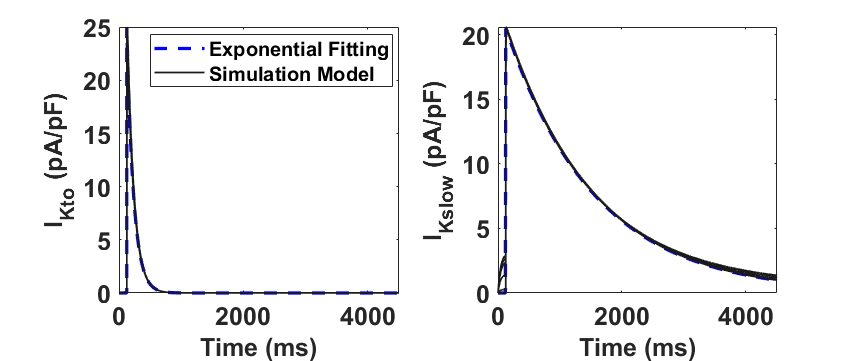
\includegraphics[width=1\linewidth]{photo/exp_sim_wt.png}}
    \\
    \subfloat[Mgat1KO]{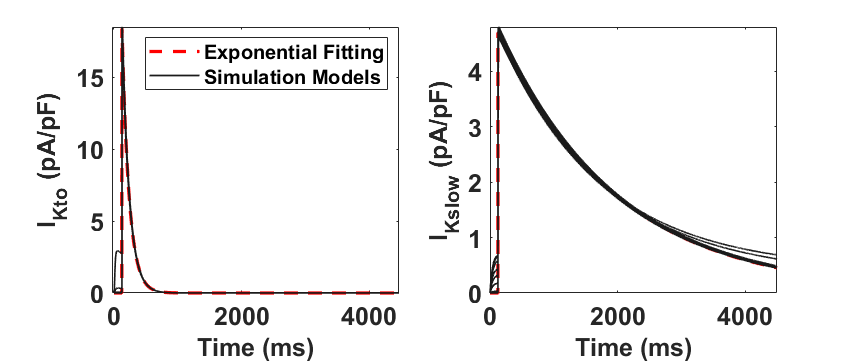
\includegraphics[width=1\linewidth]{photo/exp_sim_ko.png}}
    \caption{Current traces generated from the fitted simulations models (gray transparent line) are compared with the benchmark exponential fitting (blue and red dotted lines) for each group. On each plot, the 30 simulations results (gray lines) are overlapping}
\end{figure}
Fig. 6 shows the current traces generated by the calibrated simulation models and exponential models with the mean amplitudes and time constants from in-vitro experiment data. Simulation models are shown to be compatible with results of exponential fitting in the electrophysiological data. The solid gray lines represent simulated current traces with 30 repetitions. Except for $\text{I}_{Kslow}$ of the Mgat1KO, it is difficult to distinguish the two traces through a visual inspection. For this one, there was a slight dissimilarity during the early decay phase. Also, before applying the clamp voltage, it showed instability that currents had small positive values under the holding potential. Due to the small peak but large time constant, the trace of the Mgat1KO is flattened compared to a typical decaying exponential function, which sharply decreases after the peak. This change is expected to show modeling differences between WT and Mgat1KO.

\subsection{Simulation to Compare WT and Mgat1KO}
\begin{figure}
    \label{fig 7}
    \centering
    \subfloat[WT]{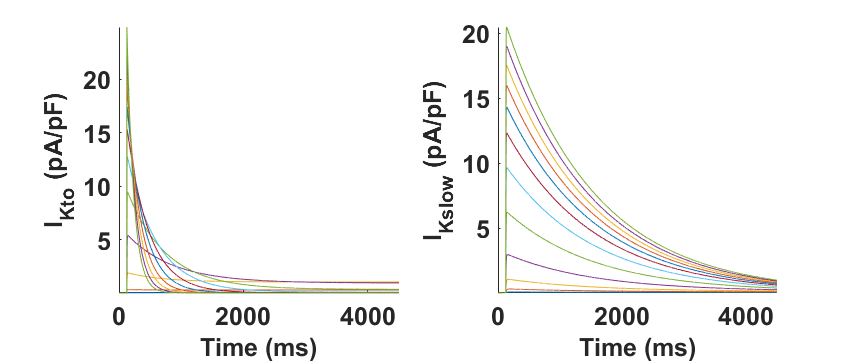
\includegraphics[width=1\linewidth]{photo/trc_wt.png}}
    \\
    \subfloat[Mgat1KO]{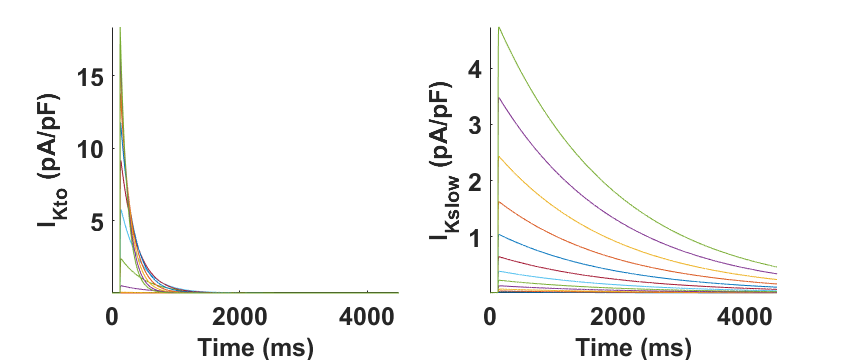
\includegraphics[width=1\linewidth]{photo/trc_ko.png}}
    \caption{Simulated current traces of the two component $\text{K}^{+}$ currents for each group. (a) Current traces of the WT group and (b) for the Mgat1KO group. Clamp voltages of 4.5 seconds were applied to between -60 mV to +50 mV by 10-mV increments from the holding potential -70 mV.}
\end{figure}
To further investigate additional differences between the Mgat1KO and WT groups, current traces were simulated at voltages between -60 mV and 50 mV in 10-mV increments as shown in Fig. 7. Simulated current traces show different patterns as voltage changes between two groups. For $\text{I}_{Kslow}$ in Fig. 7, as voltage decreases, the amplitude declines rapidly, for Mgat1KO, while reducing evenly in WT. Because of the rapid reduction, $\text{I}_{Kslow}$ traces for Mgat1KO below 0 mV depolarizations are negligible. In addition, from the perspective of decay phase, the current decreases slowly for $\text{I}_{Kslow}$ in the Mgat1KO group. It is predicted that there are differences in conductance values between the two groups.

\begin{figure}
    \label{fig 8}
    \centering
    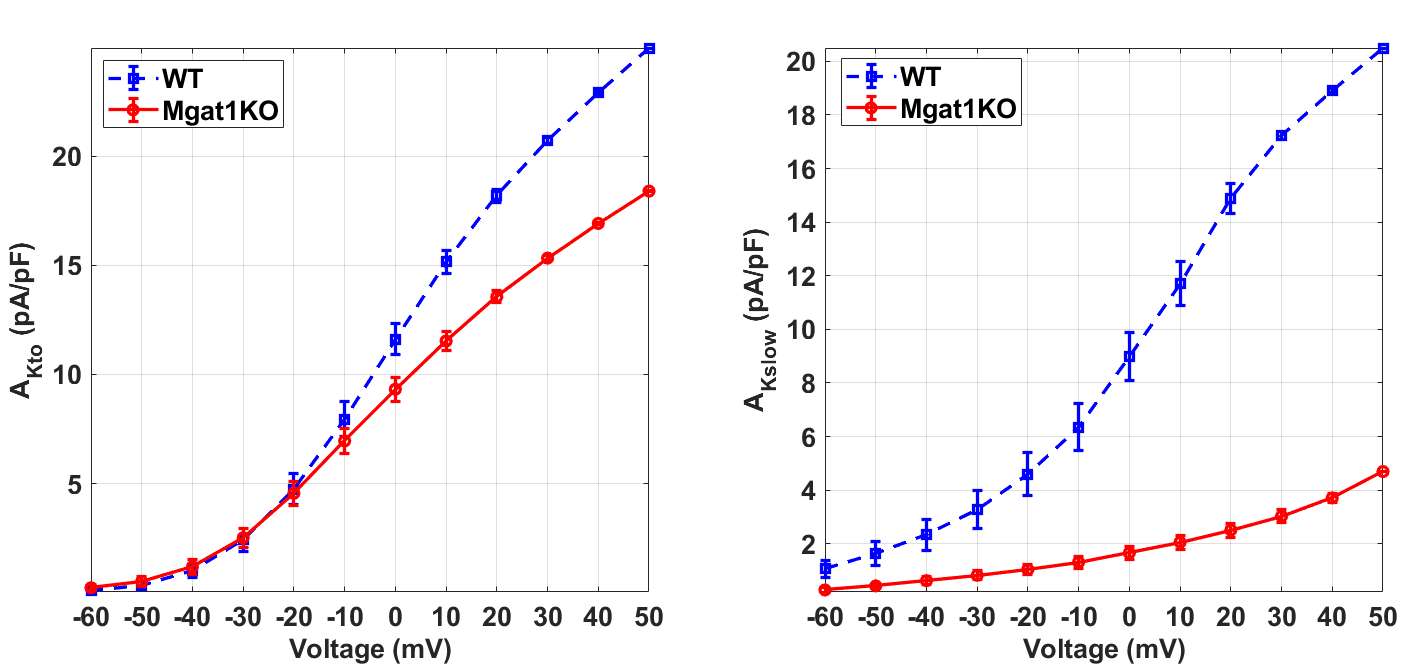
\includegraphics[width=1\linewidth]{photo/A-V.png}
    \caption{The prediction of the current density to voltage relationship for $\text{I}_{Kto}$ and $\text{I}_{Kslow}$ under Mgat1KO (red solid line with circle markers) and WT conditions (blue dotted line with square markers). Amplitudes (peaks of traces) were recorded for voltage steps ranging from -60 mV to 50 mV by 10-mV increments.} 
\end{figure}
Fig. 8 further demonstrates the differences in predicted current-density with voltage between WT and Mgat1KO. For both $\text{I}_{Kto}$ and $\text{I}_{Kslow}$, channels responsible for the two current types are less  active at a given depolarized activation voltage compared to the WT. The difference in the current peaks between the two groups is more prominent at depolarizations beyond -10 mV. This gap is significant in the $\text{I}_{Kslow}$. At all voltages, the Mgat1KO $\text{I}_{Kslow}$ is smaller than the WT $\text{I}_{Kslow}$. This is consistent with in-vitro experimental results in which the average amplitude of $\text{I}_{Kto}$ and $\text{I}_{Kslow}$ were significantly reduced with N-glycosylation perturbation (in the Mgat1KO), and the reduction in Mgat1KO $\text{I}_{Kslow}$ was bigger than for Mgat1KO $\text{I}_{Kto}$. 

\begin{figure}
    \label{fign 9}
    \centering
    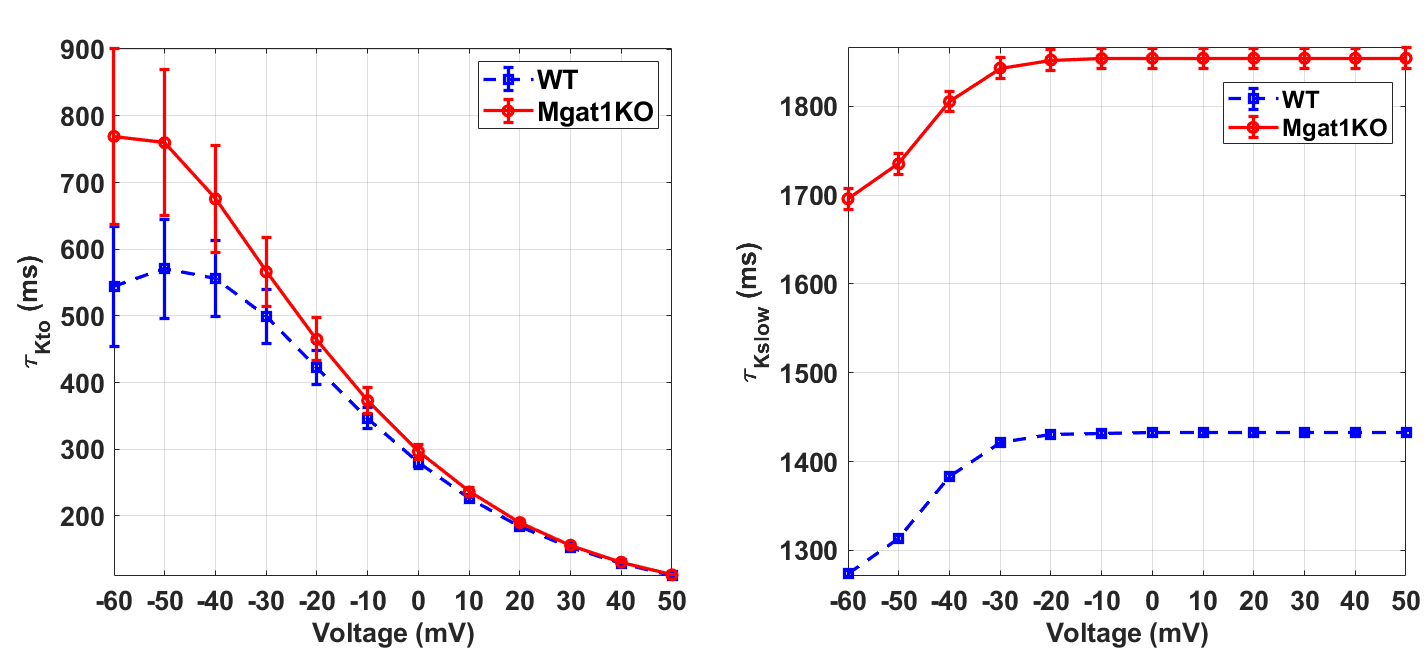
\includegraphics[width=1\linewidth]{photo/tau-V.png}
    \caption{The prediction of inactivation time constants for $\text{I}_{Kto}$ and $\text{I}_{Kslow}$ with voltage steps from -60 mV to 50 mV by 10 mV steps.} 
\end{figure}
To investigate the inactivation gating mechanism, inactivation time constants at various voltages were simulated as shown in Fig. 9. $\tau_{Kto}$ does not show a significant difference between Mgat1KO and WT when the depolarization is greater than -20 mV. There are gaps in the case where voltages are less than -20 mV, but the uncertainty represented by the error bars are too wide to make reliable predictions. $\tau_{Kslow}$ shows consistent differences, with the Mgat1KO inactivating significantly more slowly than WT at all voltages. Fig. 10 provides further information of the steady-state inactivation (SSI) rate. The SSI relationships are not significantly different between Mgat1KO and WT for either current type. These data, the longer transition times from open to inactivated state and the lack of a shift in the voltage dependence of $\text{K}_{v}$ distribution between open and inactivated states (SSI) for less glycosylated $\text{K}_{v}$ (Mgat1KO), are consistent with our previous studies \cite{schwetz2010n, ednie2015reduced, du2017}

\begin{figure}
    \label{fig 10}
    \centering
    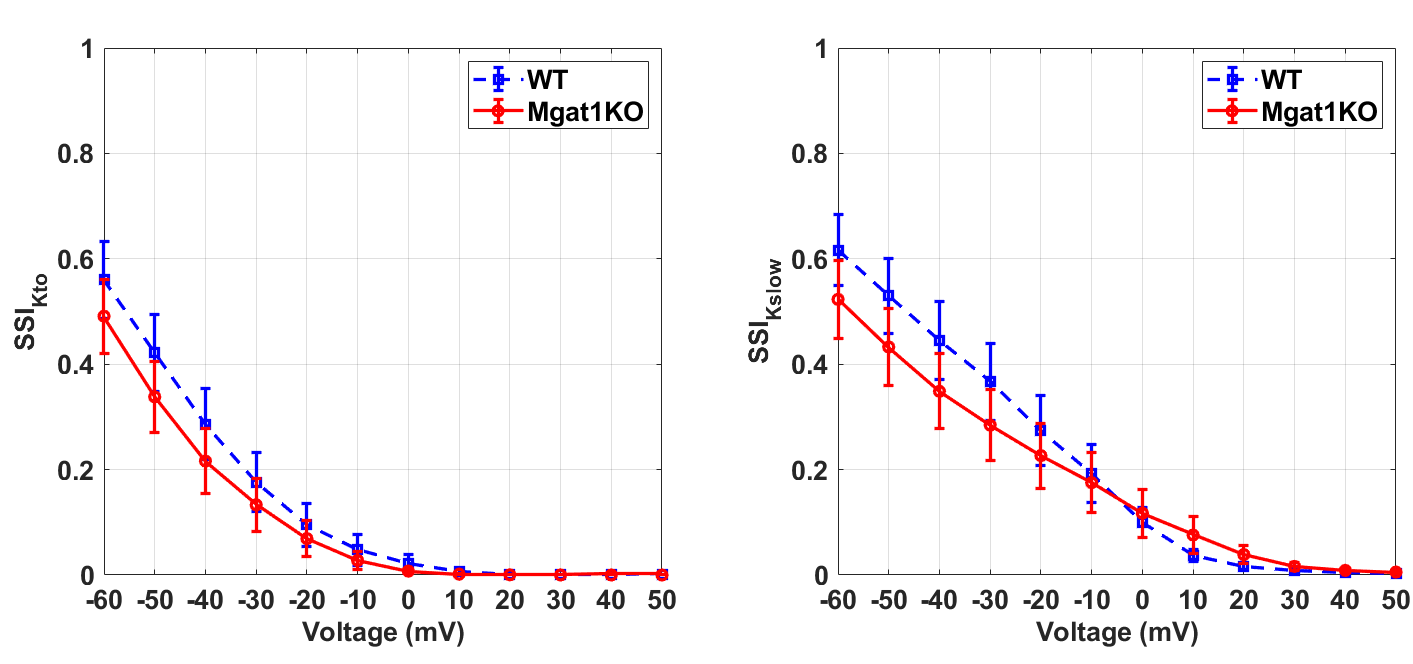
\includegraphics[width=1\linewidth]{photo/SSI-V.png}
    \caption{The prediction of SSI for $\text{I}_{Kto}$ and $\text{I}_{Kslow}$ with voltage steps from -60 mV to 50 mV by 10 mV steps.} 
\end{figure}

% === CONCLUSION ========================================================
% =======================================================================
\section{Conclusions}
This paper has developed a self-breeding GA method to build simulation models of voltage-gated $\text{K}^{+}$ channel of mouse ventricular apex myocytes from key statistics and raw data obtained from in-vitro whole cell voltage-clamp experiments \cite{ednie2019reduced}. Amplitude and time constant when the peak of a current trace decays by $e^{-1}$ are the key statistics to calibrate the simulation models. In-silico simulation models allow for the investigation of underlying dynamics of observed current and to make inferences about different experimental conditions that were not yet or cannot be conducted.

Notably, ventricular myocyte $\text{I}_{K}$ is produced through the activity of several $\text{K}_{v}$ isoforms so that there are multiple component currents corresponding to the total $\text{I}_{Ksum}$. However, only the sum of the component currents can be recorded during in-vitro experiments. Typically, the sum of potassium currents is approximated by fitting the sum of exponential functions. The exponential model gives amplitudes and time constants for each component current. Although they describe the shape of current waveform relatively well, they cannot adequately describe detailed kinetics.

Simulation models were evaluated by comparing their simulated current traces with those derived from the exponential decomposition of $\text{I}_{Ksum}$. The simulation models made it possible to predict characteristics of $\text{K}_{v}$'s at different voltages that were not conducted in the electrophysiological experiments. In addition to the changes in amplitudes and time constants for Mgat1KO group at 50 mV voltage, the simulation models predicted changes of amplitudes, time constants, and SSI with different voltages that were consistent with previous studies \cite{ednie2019reduced}.

Results show that the proposed optimization method was able to build simulation models of $\text{K}_{v}$'s compatible with the in-vitro experimental results. With these simulations models, potassium current traces at different experimental conditions and varying membrane potentials were simulated. It is predicted that in the Mgat1KO group, both $\text{I}_{Kto}$ and $\text{I}_{Kslow}$ densities are significantly reduced and the rate of $\text{I}_{Kslow}$ inactivation is much slower, which are consistent with experimental observations.

This study utilizes cardiac electrophysiology models as complementary methods to in-vitro experiments to investigate the effects of reduced N-glycosylation on $\text{K}_{v}$ activity. A new method is used to delineate and examine multiple potassium currents. The computational simulation helps demonstrate the voltage-gating mechanism and conductance kinetics that cannot be readily measured through exponential fits of whole cell $\text{K}^{+}$ currents. 

% === ACKNOWLEDGMENT ====================================================
% =======================================================================
\section*{Acknowledgment}
This research is supported by the National Science Foundation grants MCB-1856132 and MCB-1856199. Any opinions, findings, or conclusions expressed in this paper are those of the authors and do not necessarily reflect the views of the sponsor.


% if have a single appendix:
%\appendix[Proof of the Zonklar Equations]
% or
%\appendix  % for no appendix heading
% do not use \section anymore after \appendix, only \section*
% is possibly needed

% use appendices with more than one appendix
% then use \section to start each appendix
% you must declare a \section before using any
% \subsection or using \label (\appendices by itself
% starts a section numbered zero.)
%

% ============================================
%\appendices
%\section{Proof of the First Zonklar Equation}
%Appendix one text goes here %\cite{Roberg2010}.

% you can choose not to have a title for an appendix
% if you want by leaving the argument blank
%\section{}
%Appendix two text goes here.


% use section* for acknowledgement
%\section*{Acknowledgment}


% Can use something like this to put references on a page
% by themselves when using endfloat and the captionsoff option.
\ifCLASSOPTIONcaptionsoff
  \newpage
\fi


% trigger a \newpage just before the given reference
% number - used to balance the columns on the last page
% adjust value as needed - may need to be readjusted if
% the document is modified later
%\IEEEtriggeratref{8}
% The "triggered" command can be changed if desired:
%\IEEEtriggercmd{\enlargethispage{-5in}}

% ====== REFERENCE SECTION

%\begin{thebibliography}{1}

% IEEEabrv,

\bibliographystyle{IEEEtran}
\bibliography{IEEEabrv,Bibliography}
%\end{thebibliography}
% biography section
% 
%% insert where needed to balance the two columns on the last page with
%% biographies
%%\newpage
% If you have an EPS/PDF photo (graphicx package needed) extra braces are
% needed around the contents of the optional argument to biography to prevent
% the LaTeX parser from getting confused when it sees the complicated
% \includegraphics command within an optional argument. (You could create
% your own custom macro containing the \includegraphics command to make things
% simpler here.)
%\begin{biography}[{\includegraphics[width=1in,height=1.25in,clip,keepaspectratio]{mshell}}]{Michael Shell}
% or if you just want to reserve a space for a photo:

% ==== SWITCH OFF the BIO for submission
% \begin{IEEEbiography}[{\includegraphics[width=1in,height=1.25in,clip,keepaspectratio]{photo/haedong_low.jpg}}]{Haedong Kim}
% Turn off for submission
% \end{IEEEbiography}
% \begin{IEEEbiography}[{\includegraphics[width=1in,height=1.25in,clip,keepaspectratio]{photo/haedong_low.jpg}}]{Hui Yang}
% Turn off for submission
% \end{IEEEbiography}
% \begin{IEEEbiography}[{\includegraphics[width=1in,height=1.25in,clip,keepaspectratio]{photo/haedong_low.jpg}}]{Andrew R. Ednie}
% Turn off for submission
% \end{IEEEbiography}
% \begin{IEEEbiography}[{\includegraphics[width=1in,height=1.25in,clip,keepaspectratio]{photo/haedong_low.jpg}}]{Eric S. Bennett}
% Turn off for submission
% \end{IEEEbiography}

% You can push biographies down or up by placing
% a \vfill before or after them. The appropriate
% use of \vfill depends on what kind of text is
% on the last page and whether or not the columns
% are being equalized.

\vfill

% Can be used to pull up biographies so that the bottom of the last one
% is flush with the other column.
%\enlargethispage{-5in}
\end{document}
